\begin{figure}[htbp]
	\centering
	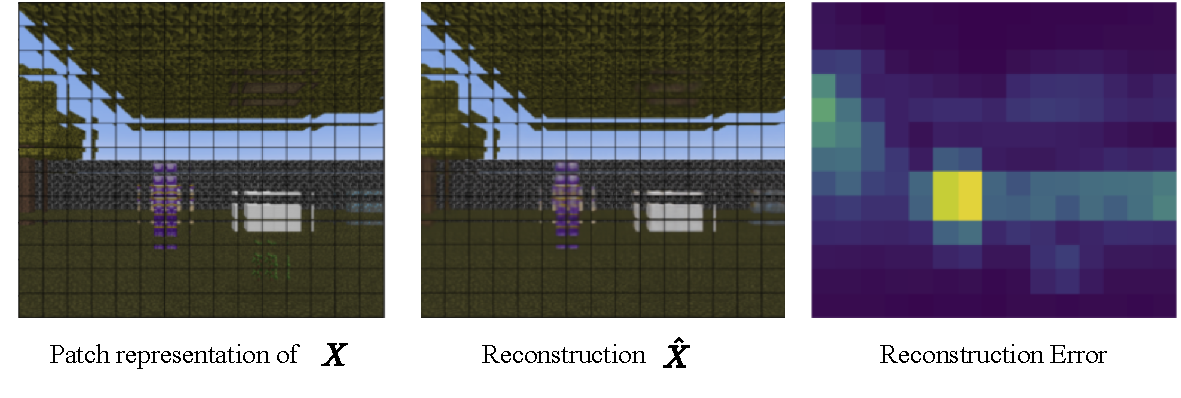
\includegraphics[width=0.85\textwidth]{figures/chapter5/vision_patches.pdf}
	\caption{Input and output example from the patch-based autoencoder of the agent's vision model. The image $X$ obtained through the domain interface (left) is segmented into patches and reconstructed by the autoencoder (middle). The per-patch reconstruction error (right) is used as a novelty signal, with higher values (lighter) indicating regions more likely to contain unknown visual elements.}
	\label{fig:vision_fig}
\end{figure}
